\documentclass[11pt,aspectratio=169]{beamer}
\graphicspath{{Images/}{./}}
\usepackage{booktabs}
\usepackage{tikz}
\usepackage[export]{adjustbox}
\usepackage{caption}
\usepackage{fontspec}
\setmainfont{Noto Serif}
\newfontfamily\devanagari{Noto Serif Devanagari}[Script=Devanagari]
\newfontfamily{\iast}{Noto Serif}[Mapping=itrans-iast]
\usetheme{Madrid}
\definecolor{teal}{RGB}{8,88,88}
\setbeamercolor*{structure}{bg=teal!20,fg=teal!90}
\setbeamercolor*{palette primary}{use=structure,fg=white,bg=structure.fg}
\setbeamercolor*{palette secondary}{use=structure,fg=teal,bg=white}
\setbeamercolor*{palette tertiary}{use=structure,fg=white,bg=myBlue} 
\setbeamercolor{frametitle}{bg=teal!85,fg=white}
\setbeamertemplate{footline}{}
\setbeamertemplate{navigation symbols}{}
\setbeamercolor*{titlelike}{parent=palette primary}
\setbeamercolor{section in head/foot}{fg=teal, bg=white}
\setbeamercolor{item projected}{bg=teal}
\setbeamertemplate{enumerate items}{bg=teal}
\setbeamercolor{itemize item}{fg=teal}
\setbeamercolor{itemize subitem}{fg=teal}
\setbeamercolor{button}{bg=teal}
\setbeamercolor{section in toc}{fg=black}
\setbeamercolor{subsection in toc}{fg=black}
\setbeamercolor{block title}{bg=teal, fg=white}
\setbeamercolor{block body}{bg=teal!20}
\useinnertheme{circles}
\useoutertheme{miniframes}
\setbeamertemplate{headline}{}
\title{Aspirations in the Air: Effect of Development \\ Schemes on AQI}
\subtitle{Evidence from a Spatial RD in India}
\author{Aayushi Agarwal, Bhaskar Agarwal, Gaurav Banerjee, Nandish Patel}
\date{\today}
\begin{document}

\section{}
\begin{frame}
\titlepage
\end{frame}
\setbeamertemplate{headline}[miniframes theme]

\begin{frame}
\frametitle{Contents}
\begin{itemize}
\item Background: Why study development reforms in the context of air quality?, Common problems, Exogenous variation...
\item Methodology: Sources of data, Wrangling, Merging, Cleaning
\item Empirical strategy: Identification, Model, Controls
\item Results: State-wise, Aggregated, Placebo Test
\item Conclusion: Shortcomings, Way ahead, Q/A
\end{itemize}
\end{frame}

\section{Background} 
\begin{frame}{Why look at development schemes?}
\begin{block}{Mechanism I}
AQI = $\downarrow$ f(Development)
\end{block}
\begin{itemize}
\item Clean Cooking Adoption
\item Waste Management
%\item<5-> \devanagari{यतः परस्परं विवदमानानाम् अपि धर्मशास्त्राणाम् \textbf{अहिंसा परमो धर्म} इत्यत्रैकमत्यम् ।}
\item Agricultural Residue Management
\end{itemize}
\end{frame}

\begin{frame}{On the other hand...}
\begin{block}{Mechanism II}
AQI = $\uparrow$ f(Development)
\end{block}
\begin{itemize}
\item Infrastructure Development
\item Increased Industrial Output 
\item Rise in Vehicular Emission 
\end{itemize}
Finding the direction of the effect is then an empirical problem
\end{frame}

\begin{frame}{Exogenous variation}
\begin{columns}
\column{0.5\textwidth}
\begin{minipage}[t][.5\textheight][t]{\textwidth}
 \centering
\begin{itemize}
\item Development policies are implemented non-randomly
\item Cannot isolate causal impact at the District level 
\end{itemize}
\end{minipage}
\column{0.5\textwidth}
\begin{minipage}[t][.5\textheight][t]{\textwidth}
 \centering
Government chooses districts to be treated \\
$\downarrow$ \\
District boundaries become treatment cutoff \\
$\downarrow$ \\
Compare subdistricts along this cutoff \\
$\downarrow$ \\
LATE using spatial regression discontinuity
\end{minipage}
\end{columns}
\end{frame}

\begin{frame}{Aspirational Districts Scheme}
\begin{itemize}
\item Launched in January 2018 by NITI Aayog
\item Aimed at rapid transformation of underdeveloped yet aspirational districts
\item Focus areas: Basic Infrastructure, Health \& Nutrition, Education, Agriculture \& Financial Inclusion
\item Selected districts using a composite deprivation index
\end{itemize}
\end{frame}


\section{Methodology}

\begin{frame}{Methodology}
\begin{block}{Research question}
``\textit{How do development policies impact subdistrict level air quality in India?}"
\end{block}
Sources of data:
\begin{itemize}
\item Master shapefile- Survey of India (SoI)
\item Treatment- NITI Aayog
\item AQI- Socioeconomic High-resolution Rural-Urban Geographic Platform (SHRUG)
\item Controls- ibid 
\end{itemize}
\end{frame}

\begin{frame}
\frametitle{Subdistricts shapefile}
 \begin{columns}
 \column{0.5\textwidth} 
\includegraphics[height= 0.8\textheight, center]{1_Total.png}
\column{0.5\textwidth}
\begin{itemize}
\item Source: Survey of India (SoI)
\item Tehsil/Taluk level administrative shapefile
\item 4723 features, 5 fields, LCC\_WGS84
\end{itemize}
\end{columns}
\end{frame}

\begin{frame}{ADS treatment status}
 \begin{columns}
 \column{0.5\textwidth} 
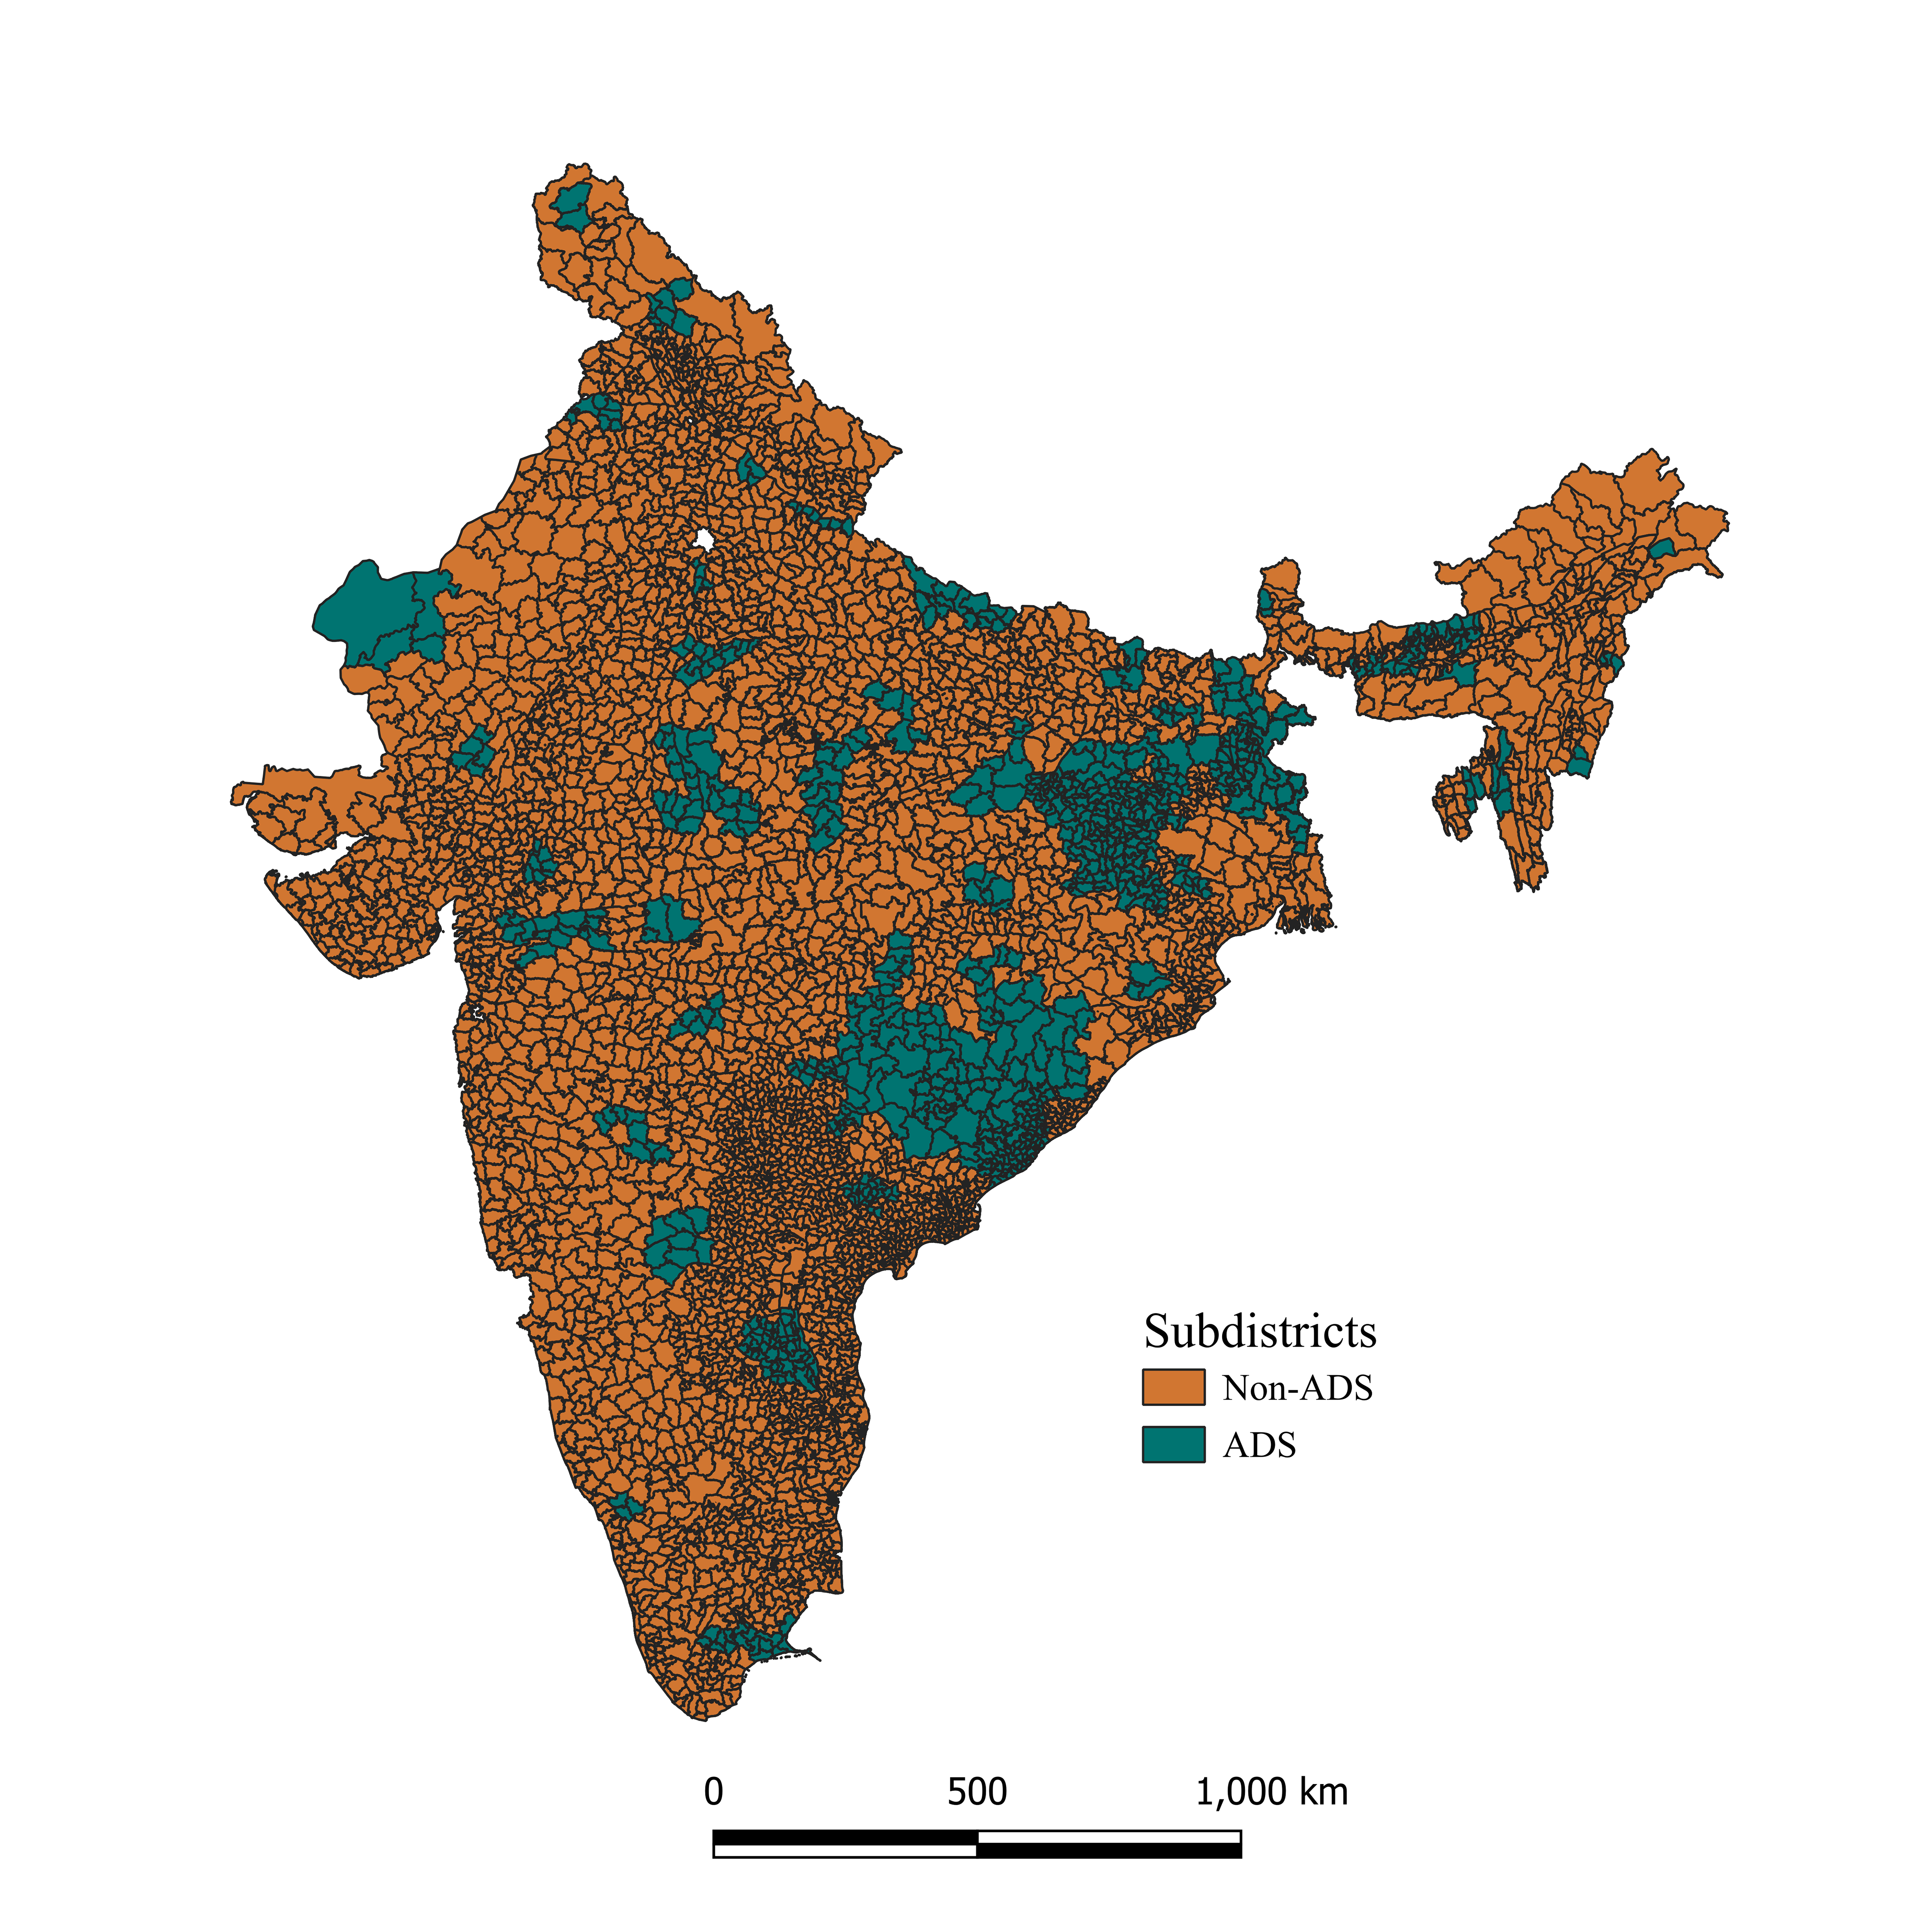
\includegraphics[height= 0.8\textheight, center]{2_TUT.png}
\column{0.5\textwidth}
\begin{itemize}
\item NITI Aayog only provides names of Districts
\item Merging areas with names is a nightmare in India- Differing spellings, Changed names...
\item As a result, we fuzzy match district names using Jaro-Winkler Distance
\item Filtered for 29 relevant states
\end{itemize}
\end{columns}
\end{frame}

\begin{frame}
\frametitle{Cutoff}
 \begin{columns}
\column{0.33\textwidth}  
\includegraphics[height= 0.7\textheight, center]{3A.png}
 \column{0.33\textwidth} 
\includegraphics[height= 0.7\textheight, center]{3B.png}
\column{0.33\textwidth}
\includegraphics[height= 0.7\textheight, center]{3C.png}
\end{columns}
\end{frame}

\begin{frame}
\frametitle{Distance to cutoff}
\includegraphics[width= 0.65\textwidth, center]{globe.jpg}
\begin{itemize}
\item `Distance to cutoff' is the perpendicular distance from centroids of subdistricts to the cutoff boundary. +ve for treated and -ve for control.
\end{itemize}
\end{frame}

\begin{frame}{AQI}
 \begin{columns}
 \column{0.5\textwidth} 
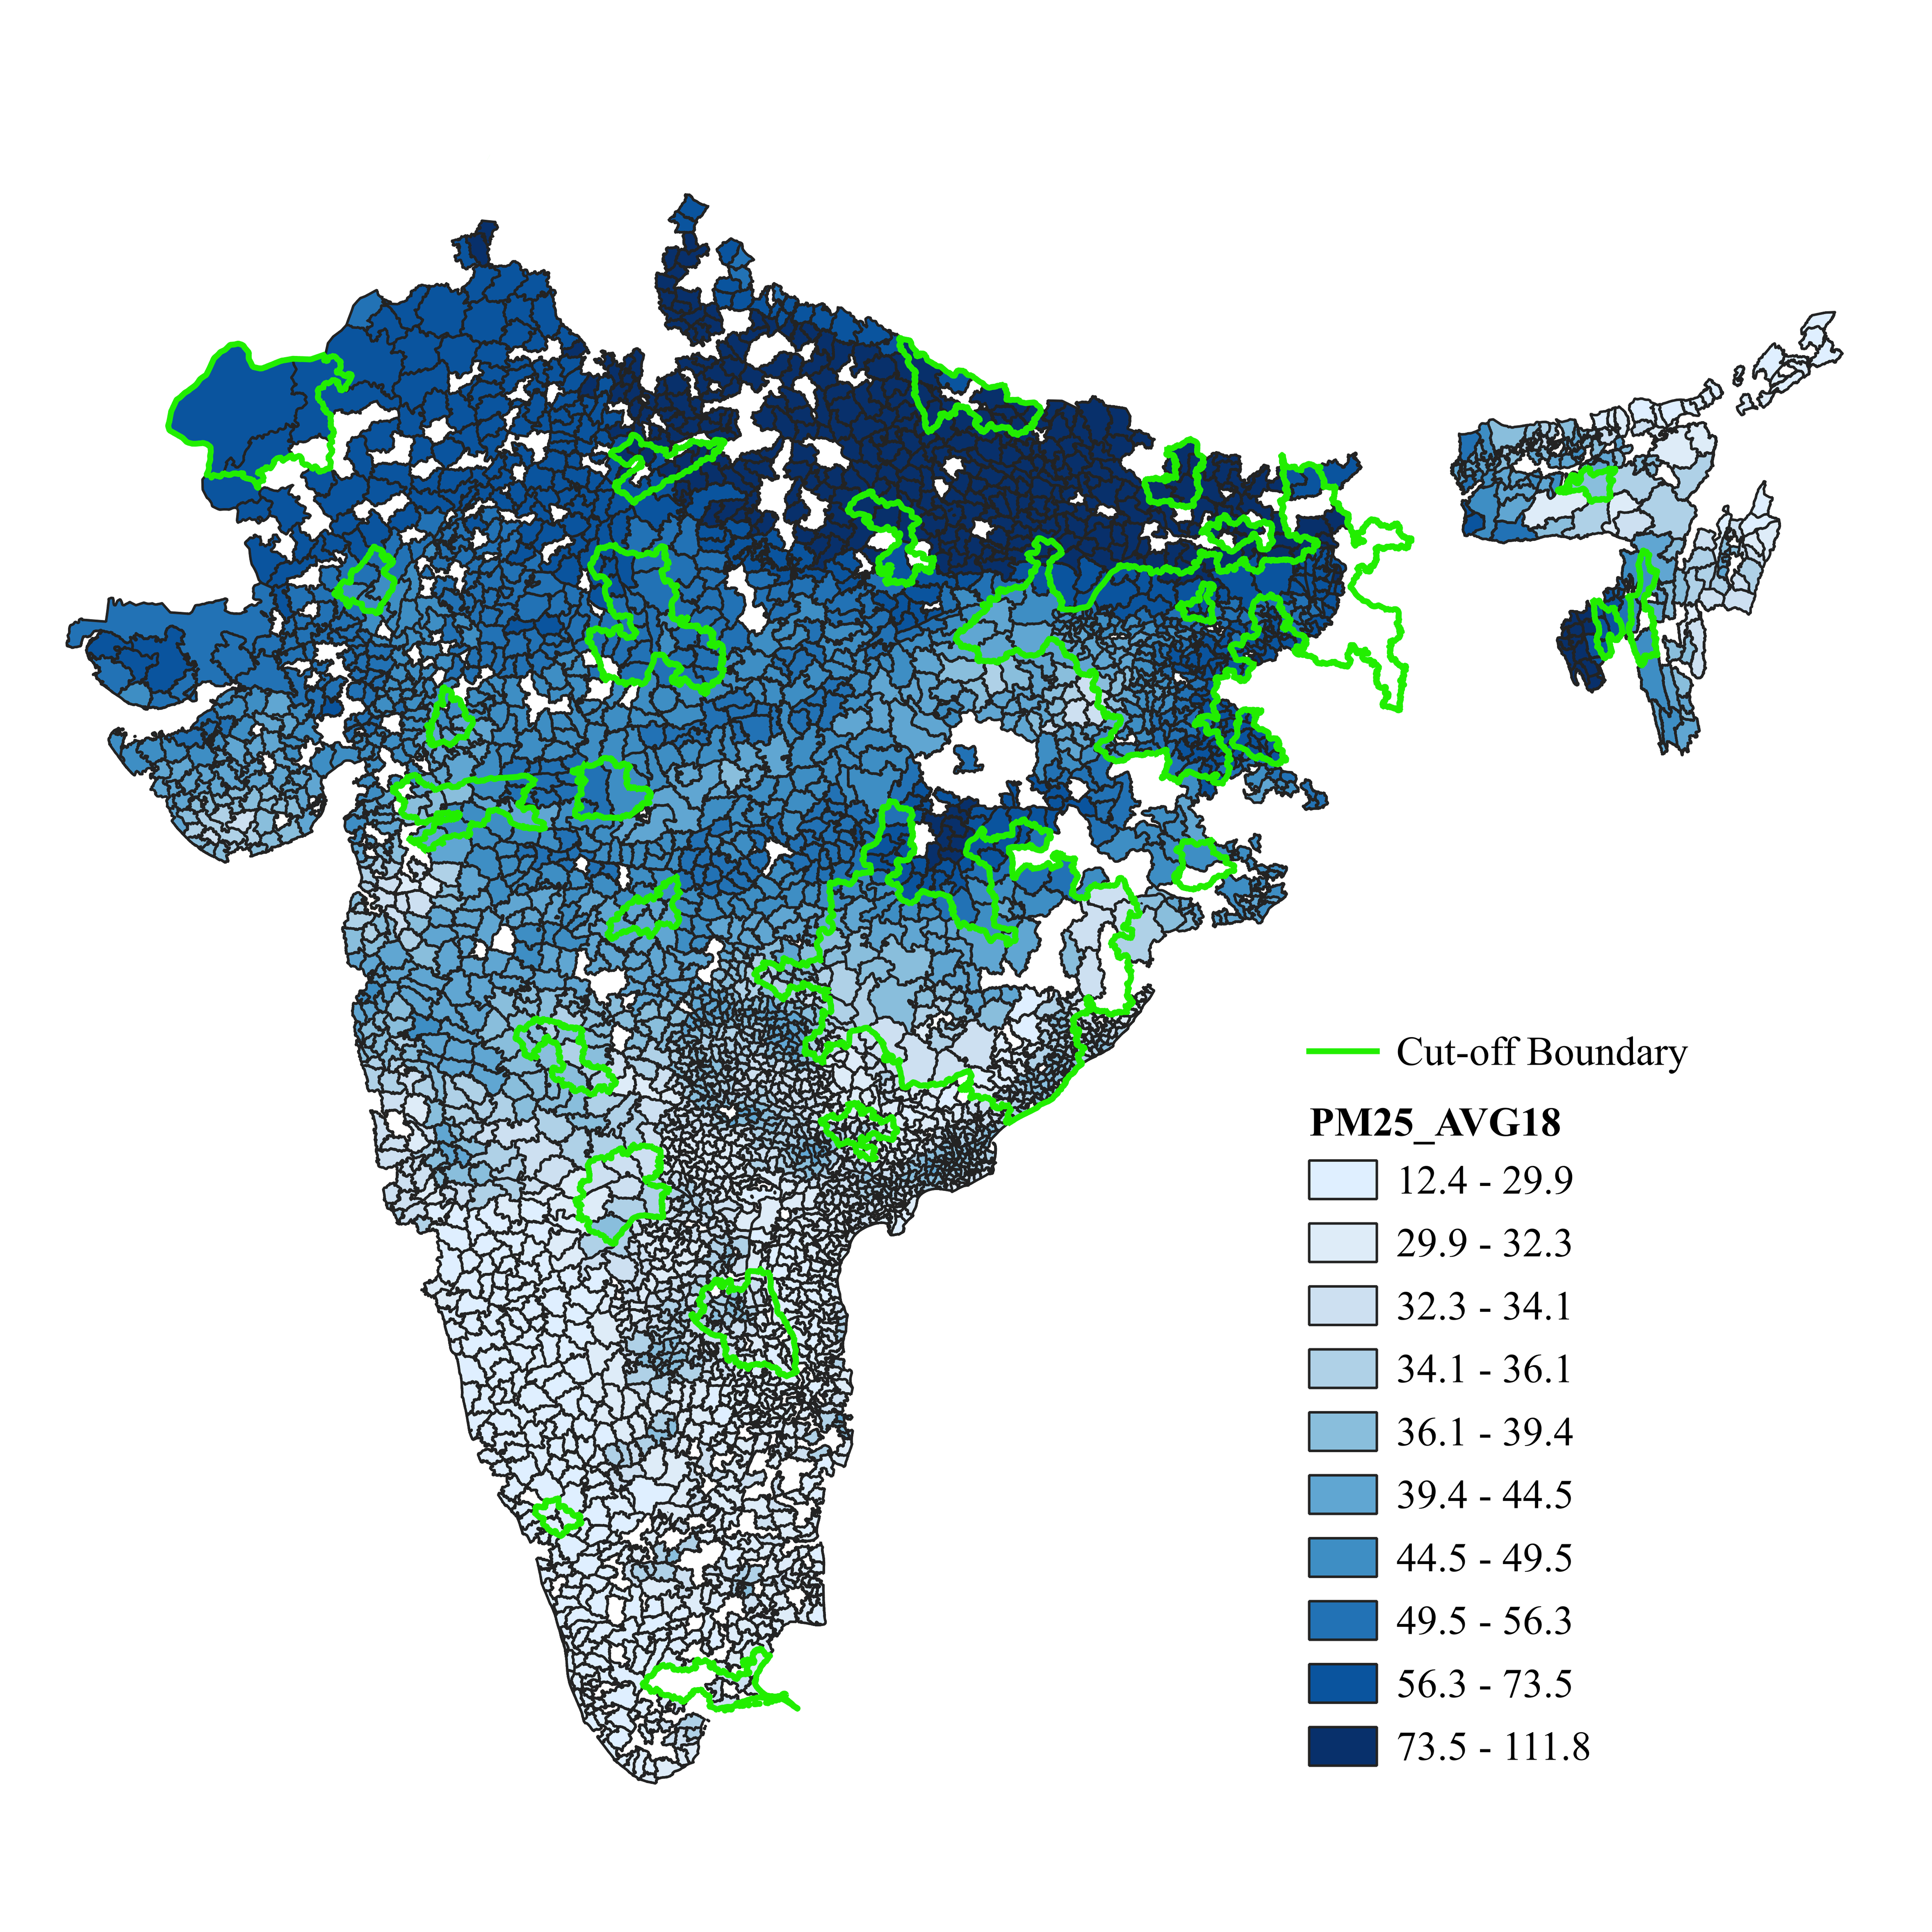
\includegraphics[height= 0.7\textheight, center]{Controls.png}
\column{0.5\textwidth}
\includegraphics[height= 0.7\textheight, center]{Jharkhand.png}
\end{columns}
\end{frame}

\begin{frame}{Why controls?}
 \begin{columns}
\column{0.5\textwidth}  
\includegraphics[height= 0.8\textheight, center]{controls_centroid.png}
 \column{0.5\textwidth} 
\begin{figure}
\includegraphics[height= 0.4\textheight, center]{theeffect.png}
\caption*{\tiny{Source: The Effect, Nick Huntington-Klein}}
\end{figure}
\end{columns}
\end{frame}

\begin{frame}{Controls}
 \begin{columns}
 \column{0.5\textwidth} 
\includegraphics[height= 0.5\textheight, center]{Merge.jpg}
\begin{table}[htbp]
\centering
\label{Controls_Post}
\begin{adjustbox}{width=0.75\textwidth}
\begin{tabular}{|l|l|c|}
\hline
\multicolumn{1}{|c|}{\textbf{\begin{tabular}[c]{@{}c@{}}S. \\ No\end{tabular}}} & \multicolumn{1}{c|}{\textbf{Controls}} & \textbf{Description} \\ \hline
1. & pc18\_sc\_share & Scheduled castes population share \\ \hline
2. & pc18\_st\_share & Scheduled tribes population share \\ \hline
3. & pc18\_lit\_share & Literate population share \\ \hline
4. & pc18\_rural\_share & Rural population share \\ \hline
5. & pc18\_work\_share & Working population share \\ \hline
6. & pc18\_forest\_share & Forest cover share \\ \hline
\end{tabular}
\end{adjustbox}
\end{table}
\column{0.5\textwidth}
\begin{itemize}
\item Source: SHRUG, PC01 and PC11
\item Extrapolation:
\begin{equation*}
\begin{adjustbox}{width=0.55\textwidth}
Growthrate_{ij} = \frac{PC11_{ij} - PC01_{ij}}{PC01_{ij}} * 100
\end{adjustbox}
\end{equation*}
\begin{equation*}
\begin{adjustbox}{width=0.35\textwidth}
AGR_{ij} = \frac{Growthrate_{ij}}{10}
\end{adjustbox}
\end{equation*}
\begin{equation*}
\begin{adjustbox}{width=0.5\textwidth}
PC18_{ij} = PC11_{ij}\left(1 + \frac{AGR_{ij}}{100} \right)^7
\end{adjustbox}
\end{equation*}
\end{itemize}
\end{columns}
\end{frame}

\section{Empirical strategy}

\begin{frame}{Identification}
 \begin{columns}
 \column{0.5\textwidth} 
\begin{figure*}
\begin{adjustbox}{width=\textwidth}
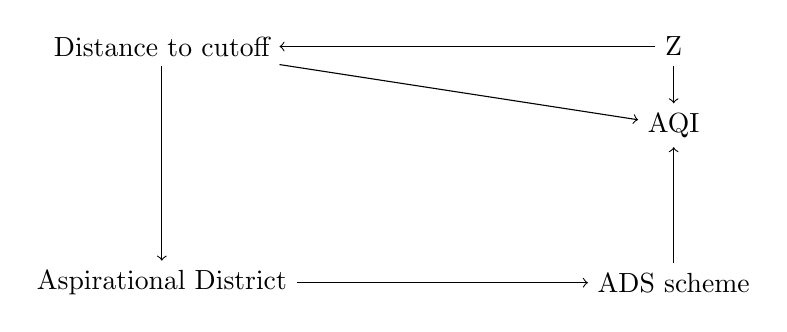
\begin{tikzpicture}
\node (v0) at (-1.5,0) {Aspirational District};
\node (v1) at (5,0) {ADS scheme};
\node (v2) at (5,2) {AQI};
\node (v3) at (-1.5,3) {Distance to cutoff};
\node (v4) at (5,3) {Z};
\draw [->] (v1) edge (v2);
\draw [->] (v0) edge (v1);
\draw [->] (v3) edge (v0);
\draw [->] (v3) edge (v2);
\draw [->] (v4) edge (v3);
\draw [->] (v4) edge (v2);
\end{tikzpicture}
\end{adjustbox}
\end{figure*}
\column{0.5\textwidth}
\begin{figure}
\includegraphics[height= 0.5\textheight, center]{theeffect2.png}
\caption*{\tiny{Source: The Effect, Nick Huntington-Klein}}
\end{figure}
\end{columns}
\end{frame}

\begin{frame}{Model}
\begin{block}{Linear}
	$pm25\_avg18_{i} = \beta_{0} + \beta_{1}A_{i} + \beta_{2}D_{i} + \beta_{3}A_{i}D_{i} + \mu_{i}$
\end{block}
$\beta_{1}$ is the coefficient of interest
\begin{block}{2nd order polynomial}
	$pm25\_avg18_{i} = \beta_{0} + \beta_{1}A_{i} + \beta_{2}D_{i} + \beta_{3}{D_{i}}^2 + \beta_{4}A_{i}D_{i} + \beta_{5}A_{i}(D_{i})^2 + \mu_{i}$
\end{block}
Following the recommendations of [Gelman and Imbens, 2019], we do not check for higher order polynomials greater than two
\end{frame}

\begin{frame}{rdrobust}
\begin{itemize}
\item Bias correction
\item MSE optimised bandwidth selection
\item Triangularly weighted kernel
\item Heteroskedasticity robust standard errors
\item Controls
\item Restricting geographical area under study
\end{itemize}
\begin{block}{Estimating model with controls}
	$pm25\_avg18_{is} = \beta_{0} + \beta_{1}A_{i} + \beta_{2}D_{i} + \beta_{3}A_{i}D_{i} + X_{i}\gamma + \lambda_{s} + \mu_{i}$
\end{block}
\end{frame}

\section{Results}

\begin{frame}{Main RD estimates}
\begin{table}[htbp]
  \caption{State-wise Robust RD Estimates} 
 \label{main} 
\begin{adjustbox}{width= 0.75\textwidth}
\begin{tabular}{@{\extracolsep{5pt}} lcccccccc} 
\\[-3.5ex]\hline 
\hline \\[-1.8ex] 
 & Estimate & $95\%$ CI & Std. Error & Robust P-Value & Obs & Eff. Obs & Bandwidth & Covs \\ 
\hline \\[-1.8ex] 
ANDHRA PRADESH & $2.125$ & $[-0.772,5.021]$ & $1.478$ & $0.151$ & $635$ & $116$ & $13.515$ & Yes\\ 
ANDHRA PRADESH & $1.382$ & $[-1.813,4.577]$ & $1.630$ & $0.397$ & $635$ & $128$ & $15.345$ & No\\ 
\hline \\[-1.8ex] 
BIHAR & $14.087$ & $[-128.410,156.585]$ & $72.704$ & $0.846$ & $79$ & $11$ & $7.035$ & Yes\\ 
BIHAR & $-39.645$ & $[-110.808,31.518]$ & $36.308$ & $0.275$ & $79$ & $5$ & $5.643$ & No\\ 
\hline \\[-1.8ex]  
GUJARAT & $3.702$ & $[-14.711,22.115]$ & $9.394$ & $0.694$ & $201$ & $47$ & $36.846$ & Yes\\ 
GUJARAT & $-0.989$ & $[-24.325,22.346]$ & $11.906$ & $0.934$ & $201$ & $47$ & $34.969$ & No\\ 
\hline \\[-1.8ex] 
\textbf{JHARKHAND} & $\textbf{-18.790}$ & $\textbf{[-35.527,-2.054]}$ & $\textbf{8.539}$ & $\textbf{0.028}$ & $\textbf{256}$ & $\textbf{17}$ & $\textbf{4.398}$ & \textbf{Yes}\\ 
JHARKHAND & $ -22.381$ & $ [-40.013,-4.749]$ & $ 8.996$ & $ 0.013$ & $ 256$ & $ 43$ & $ 6.602$ & No\\  
\hline \\[-1.8ex] 
MADHYA PRADESH & $3.868$ & $[-4.513,12.250]$ & $4.277$ & $0.366$ & $259$ & $77$ & $24.041$ & Yes\\ 
MADHYA PRADESH & $6.142$ & $[-2.170,14.454]$ & $4.241$ & $0.148$ & $259$ & $72$ & $21.989$ & No\\ 
\hline \\[-1.8ex] 
MAHARASHTRA & $0.746$ & $[-17.722,19.214]$ & $9.423$ & $0.937$ & $329$ & $53$ & $15.824$ & Yes\\ 
MAHARASHTRA & $-2.357$ & $[-28.844,24.129]$ & $13.514$ & $0.862$ & $329$ & $54$ & $16.327$ & No\\ 
\hline \\[-1.8ex] 
MIZORAM & $8.251$ & $[1.925,14.578]$ & $3.228$ & $0.011$ & $16$ & $15$ & $124.220$ & Yes\\ 
MIZORAM & $23.682$ & $[14.480,32.884]$ & $4.695$ & $0.000$ & $16$ & $15$ & $124.220$ & No\\ 
\hline \\[-1.8ex] 
RAJASTHAN & $29.610$ & $[-25.449,84.670]$ & $28.092$ & $0.292$ & $230$ & $45$ & $17.098$ & Yes\\ 
RAJASTHAN & $31.702$ & $[-26.159,89.562]$ & $29.521$ & $0.283$ & $230$ & $63$ & $25.969$ & No\\ 
\hline \\[-1.8ex] 
TELANGANA & $2.924$ & $[-17.674,23.522]$ & $10.509$ & $0.781$ & $429$ & $23$ & $5.165$ & Yes\\ 
TELANGANA & $-13.303$ & $[-50.241,23.636]$ & $18.847$ & $0.480$ & $429$ & $21$ & $4.833$ & No\\ 
\hline \\[-1.8ex] 
\end{tabular} 
\end{adjustbox}
\end{table}
\end{frame}

\begin{frame}{Aggregated RD estimate}
\begin{table}[!htbp] \centering 
  \caption{Aggregated Bias-corrected Robust RD Estimates} 
\label{total}
\begin{adjustbox}{width=0.75\textwidth}
\begin{tabular}{@{\extracolsep{5pt}} lcccccccc} 
\\[-3.5ex]\hline 
\hline \\[-1.8ex] 
 & Estimate & $95\%$ CI & Std. Error & Robust P-Value & Obs & Eff. Obs & Bandwidth & Covs \\ 
\hline \\[-1.8ex] 
ALL STATES & $1.829$ & $[-1.561,5.220]$ & $1.730$ & $0.290$ & $3456$ & $889$ & $20.572$ & Yes\\ 
ALL STATES & $-1.916$ & $[-17.619,13.787]$ & $8.012$ & $0.811$ & $3456$ & $1194$ & $30.659$ & No\\ 
\hline \\[-1.8ex] 
\end{tabular} 
\end{adjustbox}
\caption*{\textit{Notes}. Standard errors are clustered by state.}
\end{table}
\end{frame}

\begin{frame}{Placebo test}
\begin{table}[!htbp] \centering 
  \caption{Placebo Test} 
	\caption*{Outcome variable: PM2.5 in 2017 (before policy implementation)}
\label{placebo}
\begin{adjustbox}{width=0.75\textwidth}
\begin{tabular}{@{\extracolsep{5pt}} lcccccccc} 
\\[-3.5ex]\hline 
\hline \\[-1.8ex] 
 & Estimate & $95\%$ CI & Std. Error & Robust P-Value & Obs & Eff. Obs & Bandwidth & Covs \\ 
\hline \\[-1.8ex] 
JHARKHAND & $-17.297$ & $[-36.163,1.568]$ & $9.626$ & $0.072$ & $256$ & $29$ & $5.261$ & Yes\\ 
\hline \\[-1.8ex] 
\end{tabular} 
\end{adjustbox}
\caption*{\textit{Notes}. Standard errors are heteroskedasticity robust.}
\end{table}
\end{frame}

\section{Conclusion}

\begin{frame}{Conclusion}
\begin{itemize}
\item We find that AQI in 2018 is lower by approximately 18.79 units in Jharkhand for the treated subdistricts
\item Evidence for dual mechanism
\item Shortcomings: Spatial spillovers, Non-euclidean distance
\item Way forward: Village/Town level, Two-running variable approach
\end{itemize}
\end{frame}

\section{}
\begin{frame}[plain]
\frametitle{Fin.}
  \centering \Huge
	\textbf{Thank You :)}
\end{frame}
\end{document} 
